\section{Architecture}
\label{sec:architecture}

In this section we first clarify the \emph{application stack} we are assuming the SaaS application to have. Then we explain the different architectural approaches to implement versioning of SaaS, with \emph{multi-instance} as well as \emph{shared-instance} on the different application stack layers.

One important assumption we make for versioning is, that each tenant and therefore also all users of a tenant use the same version at the same time. Practially this means that each tenant has a dedicated migration point in which they decide to switch their version. This switch affects all their users at the same time. Users aren't allowed to individually choose their version.

\subsection{Application Stack}

\begin{wrapfigure}{r}{0.4\textwidth}
\centering
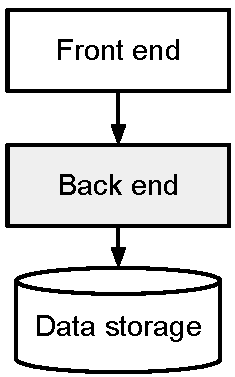
\includegraphics[]{stack.pdf}
\caption{Simplified Application Stack}
\label{fig:stack}
\end{wrapfigure}

To understand the architecture better, we first want to look at the SaaS application stack as displayed in Figure~\ref{fig:stack}. We derived this stack from our experience with developing SaaS ourselves as well as stacks we have seen in related papers (TODO references).

We assume a separation between the front-end, back-end and database layer. The \emph{front-end layer} is mainly concerned with the user interface. In a SaaS it will usually be delivered to the user's browser within a request/response cycle. Another case for the fron-end layer are native application that communicatie with the SaaS over a webservice API. We handle this more in-depth in Section~\ref{sec:sharedfrontend}. The \emph{back-end layer} is concerned with the application and business logic. It takes requests from the front-end layer and accordingly communicated with the \emph{database layer}. The front-end and back-end layers are stateless (mostly for being able to scale horizaontally). All state is kept in the database layer.

To focus our research, we omitted some details of the stack. First we were not concerned with neither caching nor load balancing. Furthermore we omitted how user management is done, especially with regards to authentication.

\subsection{Multi-Instance}

\begin{figure}
\centering
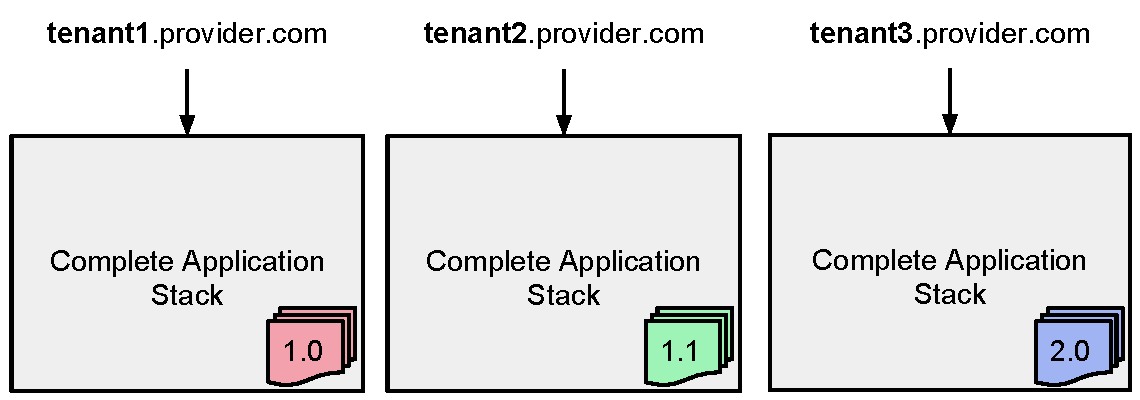
\includegraphics[width=\textwidth]{multiinstance.pdf}
\caption{Example for a version-supporting Multi-Instance Architecture}
\label{fig:multiinstance}
\end{figure}

In a multi-instance architecture the whole application stack is deployed several times on distinct resources. You can see an example in Figure~\ref{fig:multiinstance}. Usually the multi-instance architecture serves the purpose of provisioning resources for each tenant individually for horizontal scaling (TODO citation) as well as being able to develop a single-tenant application instead of having to do the engineering overhead of developing a multi-tenant application. This approach can also be used for versioning, where we see two variants:

\paragraph{Single instance per tenant} When every tenant has their own application stack instance running, these instances can be versioned by deploying the respective software version on the tentant's instance.
\paragraph{Single instance per version with multiple tenants} When every instance has a specific version, the instances in turn can be hosts for multiple tenants by using the shared-instance mechanisms explained in the following section.

Using a multi-instance architecture has the benefits that it is the most 'natural way' to provide a SaaS, since the developer does not have to deal with issues concerning multi-tenancy in one instance, like vertical scaling or isolation. Among the drawbacks are that multi-instance has a bad resource consolidation factor, thus if e.g. one tenant uses many resources but another uses none, the unused resources can't be allocated to the spiking tenant easily. Also the maintentance cost increases with the numer of tenants and there is no economy of scale working in favor of the SaaS provider here.

Versioning-wise the actual application stack is not version-aware and thus can be built without versioning as a concern. Instead versioning is handled on the deployment level. Migrations between versions might then need significant operations engineering effort.

\subsection{Shared-Instance}

The shared-instance architecture consist of one software stack deployment that serves all tenants at the same time. This architecture is the one that is generally referred to when talking about SaaS applications, since it uses the economy of scale well due to its high consolidation factor (TODO reference).

To investigate versioning in the shared-instance architecture, we will individually inspect the layers of the application stack as outlined in the previous section, consisting of the front-end, back-end and database layer. For each layer we will outline how versioning can happen. We are closing this section with a look at migrating between versions.

\subsubsection{Front-end layer}
\label{sec:sharedfrontend}

We split the \emph{front-end layer} into two categories: a \emph{web-application} running in the user's browser and an \emph{API consumer} e.g. running on the user's mobile phone.

\paragraph{Web application} In web applications the user's browser is usually reloading the whole web page on each request, which usually stems from an interaction of the user with the system\footnote{We assume that caching works transparently and perfectly as well as "One page applications" reloading their assets automatically ("hot code reload") in case something on the back-end layer changes.}. Thus there is a thight couling between the front-end and the back-end, from which we conclude that they are both versioned simultaneously. Since the front-end software is delivered to the user's browser on each request, the versioning concern can be completely handled on the \emph{back-end layer} as outlined in the next section.

\paragraph{API consumer} To allow programmatic access to the SaaS functionality, SaaS providers usually implement a webservice. A common occurance are HTTP APIs following the REST principles (TODO reference). These APIs allow native applications (e.g. mobile phone applications) or other webservices to build on top of the SaaS. The SaaS and their API consumers are loosly coupled. They follow own product cycles. In case of compatibility breaking changes in the SaaS API, the API consumers have to adapt to the changes and deploy a new version to their users. This might be hard to do e.g. because users might be reluctant to updates, delivery cycles might be too long or the API consumer developer might not have the resources to update their product. This leads us to the conclusion that SaaS APIs should be able to provide several versions of the API at the same time. The API consumer chooses which version of the API they want to use. There are many ways to handle versioning APIs and explaining them in-depth is over the scope of this report. Examples are version numbers in the URL or \emph{Accept Header} (TODO reference) of a request or feature flags for the consumer application in the SaaS (TODO reference).

  % Frontend API Versioning
  %   In URL:
  %     http://api.com/v1/resource.json?version=1
  %   Accept Header:
  %     Accept: application/json+v1
  %   Application Flag:

\subsubsection{Backend}
\paragraph{Shared-Instance 1:1}
geiles diagram

a product ver = code rev


Pro
Versioning is external to application code

Contra
heterogeneous deployment
worse consolidation factor
intelligent routing layer needed
forking of code base makes security patches difficult to apply



\paragraph{Shared-Instance 1:n}
geiles diagram


version choice is on app server


Pro
good consolidation
homogenous deployment
more flexibility: fine grained feature selection

Contra
increased code complexity
abandoning old versions needs cleanup



inside of code base are many version checks "if version == 1.4 ..."
more flexibility in choosing version, maybe not choose version but choose only features

high cost for abandoning old version to clean code base

\lstset{language=Ruby, caption=code snippet, label=code}
\begin{lstlisting}
  if(user.has_version?):
    do_something()
  end
\end{lstlisting}

\subsubsection{Database}

\paragraph{Different versions share same schema}
db is version agnostic

\paragraph{Different versions need separate schemas}
How to version schemas?

  Database needs to support several schemas for a table at the same time

  No DBMs supporting this is known to us

  Thus versioning has to happen in the backend

  \paragraph{Different tables for each schema}
  \lstset{language=SQL, caption=sql, label=sql}
  \begin{lstlisting}
    create table users_v1;
    create table users_v2;
    create table users_v3;
  \end{lstlisting}

  Pro:
  Works well if not too many versions

  Con:
  Messy design if many versions


  \paragraph{Pivot tables}

  bild von "An Elastic Multi-tenant Database Schema for Software as a Service"

  reduce dbms more to a key value store
  as used with salesforce

\subsubsection{Migration of data}
  version is chosen per tenant
  data migrations need time
  data migrations might need downtime
  on-the-fly migrations possible

